\documentclass[letterpaper,12pt]{article}
\usepackage{tabularx} % extra features for tabular environment
\usepackage{amsmath}  % improve math presentation
\usepackage{float}
\usepackage{graphicx} % takes care of graphic including machinery
\graphicspath{ {./figures/} }
\usepackage[margin=1in,letterpaper]{geometry} % decreases margins
\usepackage{cite} % takes care of citations
\usepackage[final]{hyperref} % adds hyper links inside the generated pdf file
\hypersetup{
	colorlinks=true,       % false: boxed links; true: colored links
	linkcolor=blue,        % color of internal links
	citecolor=blue,        % color of links to bibliography
	filecolor=magenta,     % color of file links
	urlcolor=blue         
}

%++++++++++++++++++++++++++++++++++++++++


\begin{document}

\title{Experiment 2 \protect\\Signal Generators and Oscilloscopes}
\author{Ahmet Akman \protect\\ Assistant : Etki Açılan}
\date{\today}
\maketitle

%\begin{abstract}
%abstract
%\end{abstract}


\section{Introduction} 
In this experiment, as students, we are expected to experiment with how to use the function generators and oscilloscopes by completing the steps described in the second experiment laboratory manual. Throughout these steps, the monitoring properties of the oscilloscope, different output forms of the signal generator are observed via connecting the instruments directly to each other and the circuit. The results of the steps were noted and plotted for further comments.

\section{Experimental Results}
In this section, the results of Experiment 2 are discussed.
\subsection{Step 1}
In this step, only the oscilloscope instrument was used. The probes of "Channel 1" are connected to the "Prob Comp" terminals which supply square waveform. After adjusting the monitor scale using the "AutoScale" button, peak to peak value is observed from the grids of the monitor. Peak to peak voltage is measured as "2.40 Volts". 'When the "Vertical Division Control" rotary button adjusted to different positions the voltage values of which the grids represents differs. When "Vertical Position Control" rotary button adjusted to diferent positions the signal moves in vertical position without changing its from. The "Horizontal Division Control" rotary button is used to scale the time steps for the active signal. The "Horizontal Position Control" is used to regulate the delay of the signal display. By observing the channel axis control buttons' functions, step 1 is completed
\subsection{Step 2}
In Step 2, the oscilloscope and probing setup is conserved as described in Step 1. After making sure channel one is activated, the substeps of a. and b. followed.
\subsubsection{a.}
The coupling method is adjusted using the on-screen menu. The difference between the "DC" and "AC" coupling methods is observed from the square waveform. As given in the figure "AC" coupling method ignores the DC component of the signal. Unlike the "DC" setting, the "AC" setting is especially used for the change on the waveform.
\begin{figure}[H]
	\caption{AC Coupling Plot}
	\centering
	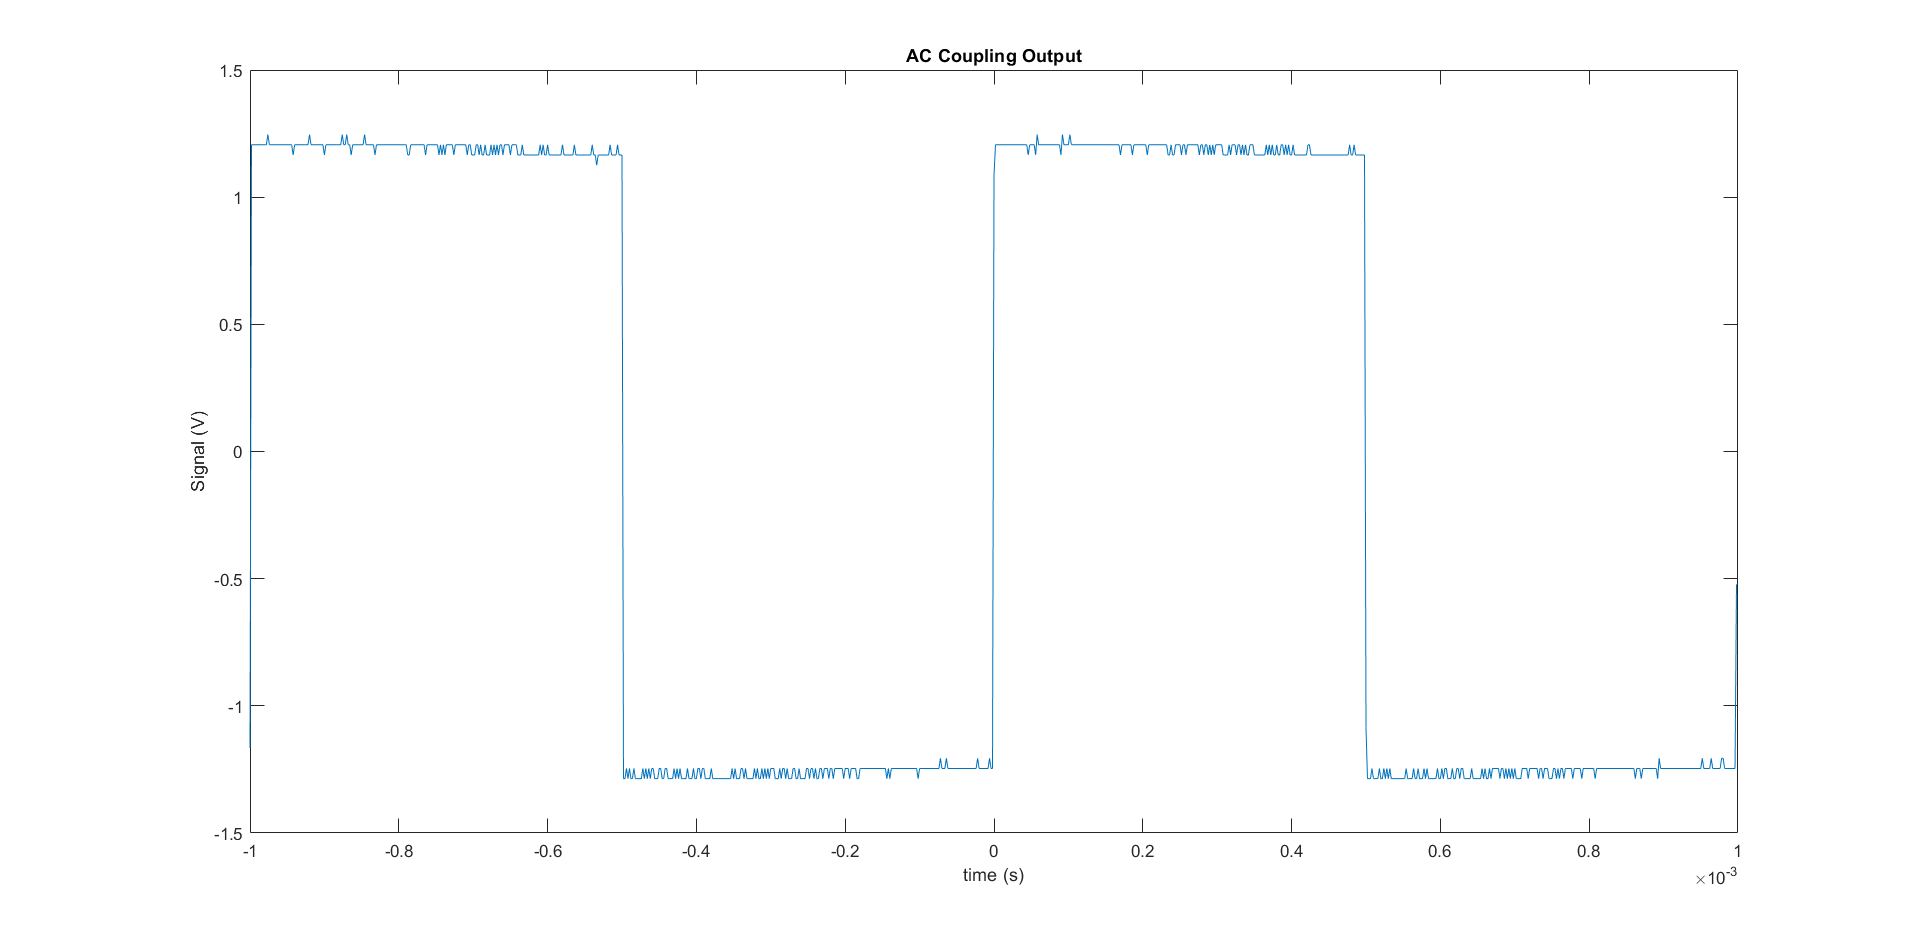
\includegraphics[width=1\textwidth]{2a.png}
\end{figure}

\subsubsection{b.}
The coupling method is adjusted using the on-screen menu, and the DC-coupled waveform is inverted. The plot of the DC-coupled signal is shown in Figure 2.

\begin{figure}[H]
	\caption{DC Coupling Plot}
	\centering
	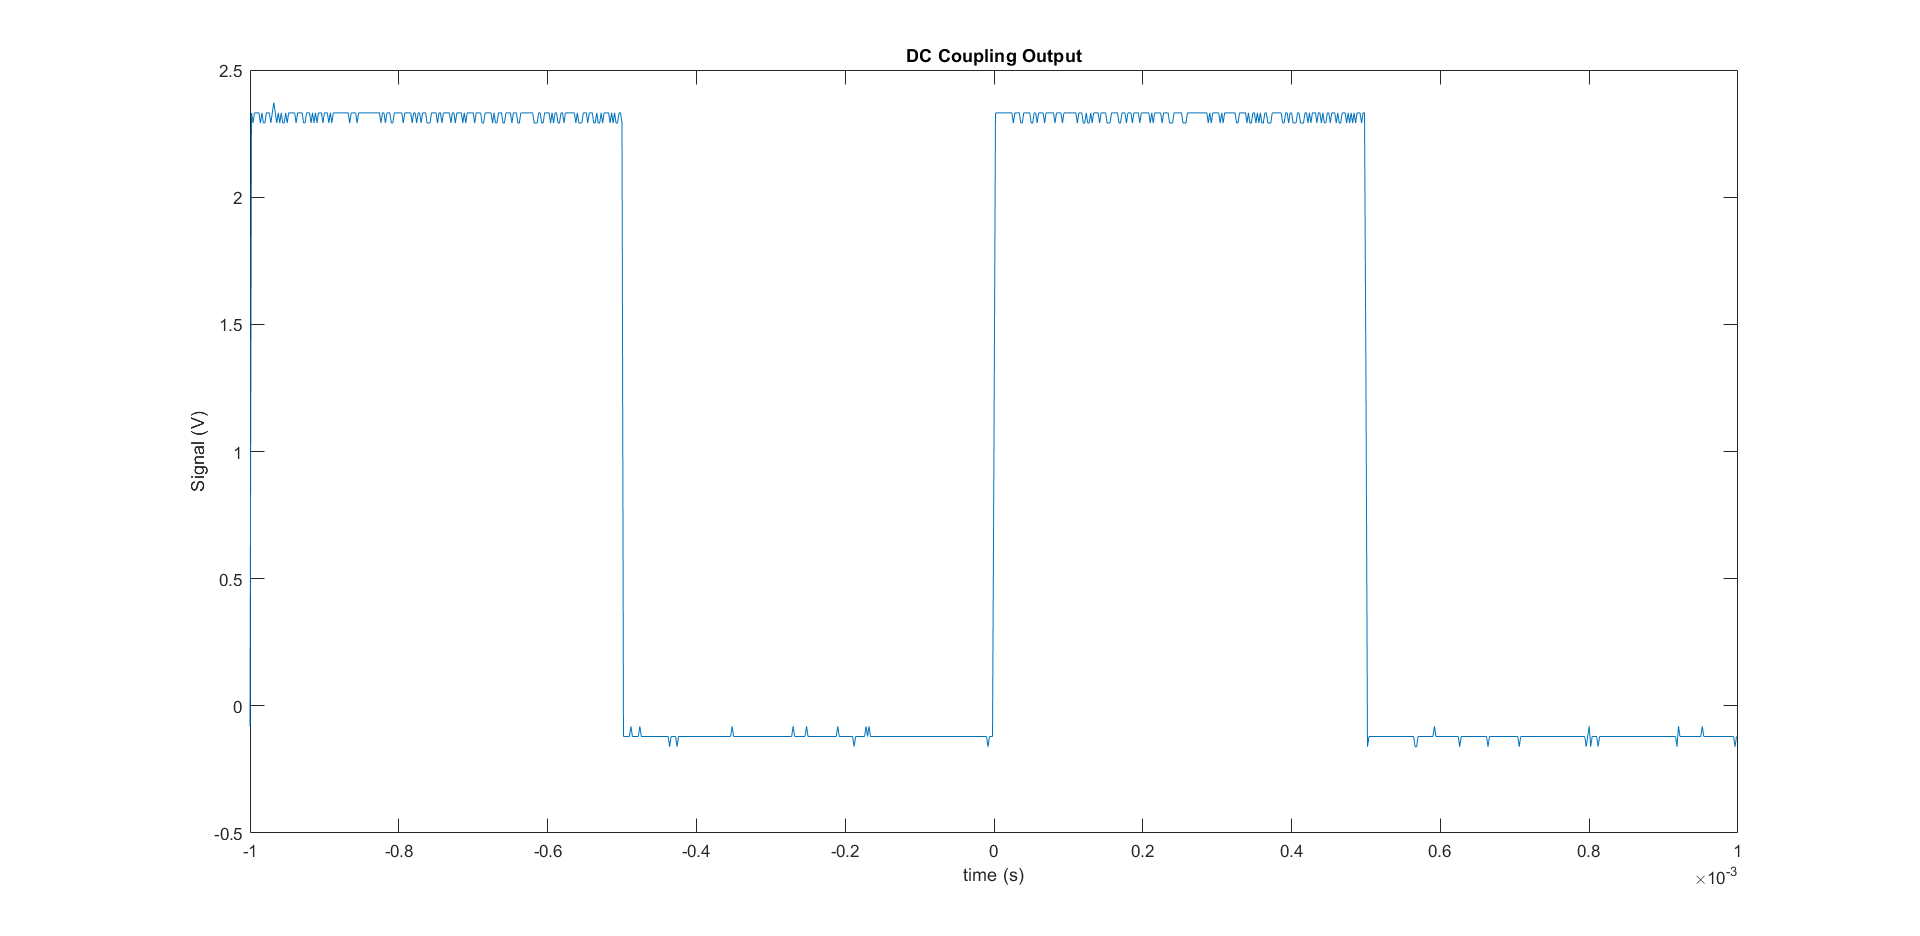
\includegraphics[width=1\textwidth]{2b1.png}
\end{figure}
The inverted form of the DC-coupled signal is observed. The plot of the inverted form is shown in Figure 3.

\begin{figure}[h]
	\caption{DC Coupling Inverted Plot}
	\centering
	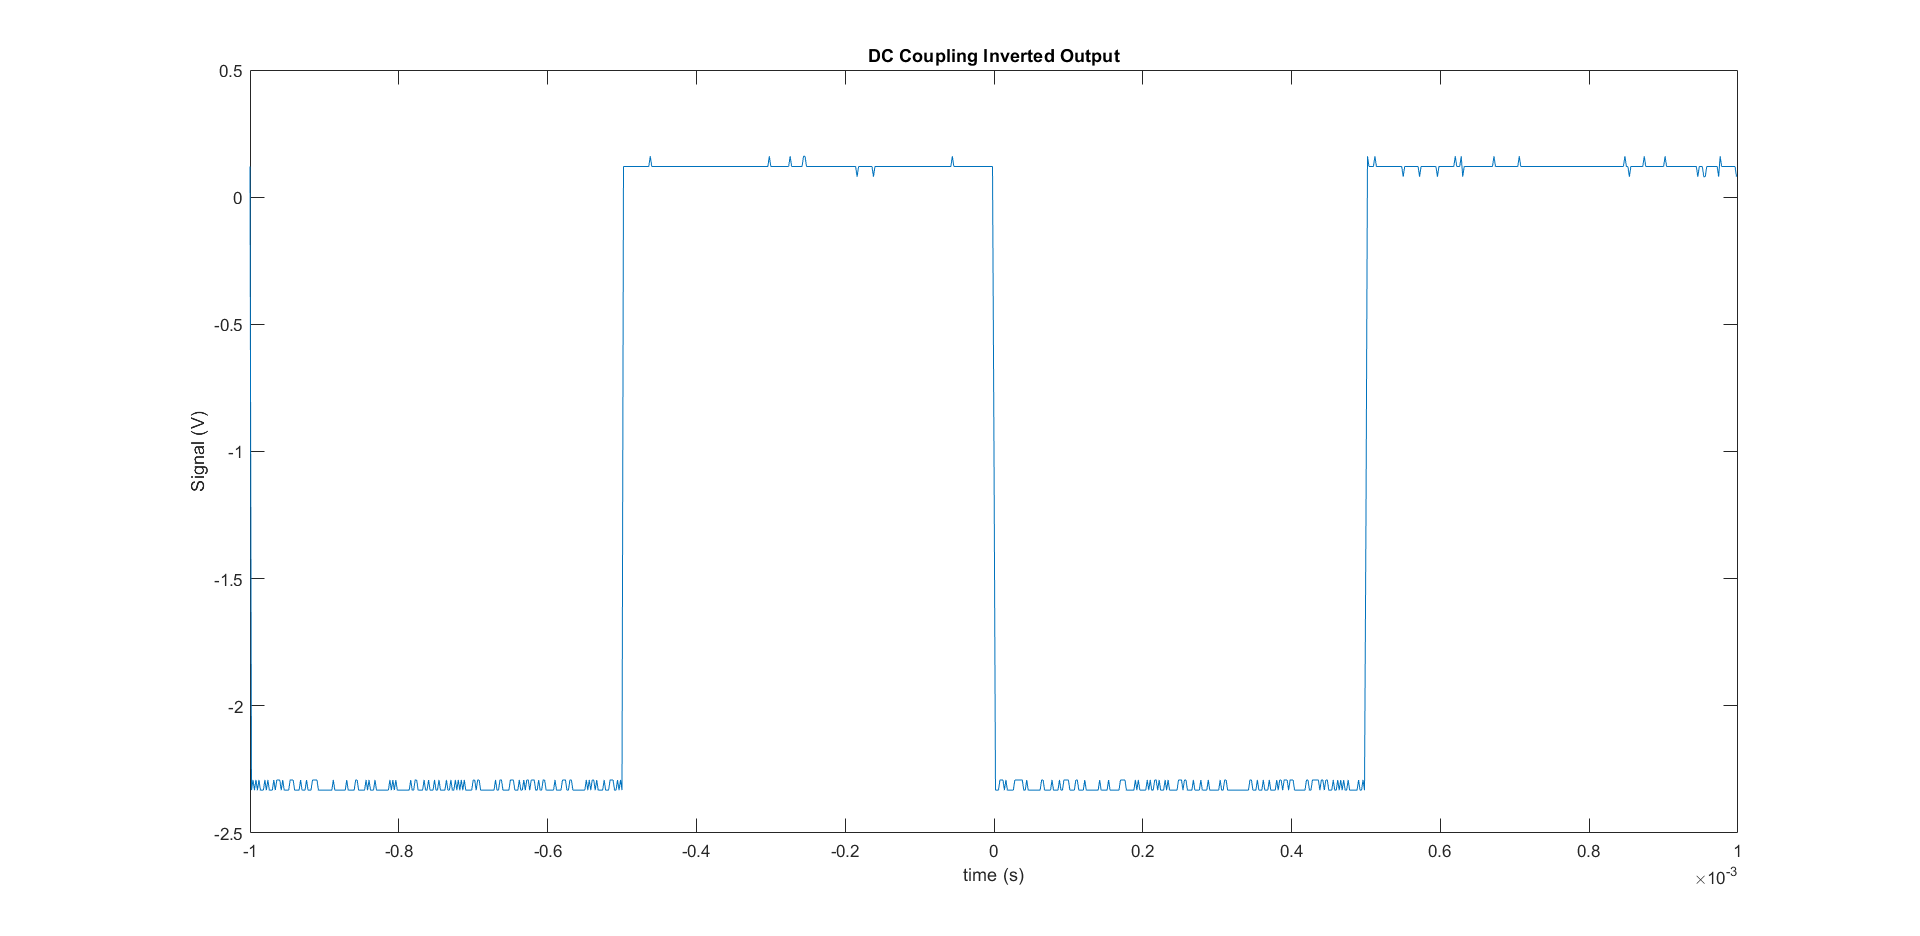
\includegraphics[width=1\textwidth]{2b2.png}
\end{figure}
When the signal is inverted, the inverse of the measured values becomes displayed so that the values are multiplied with -1. 

\subsection{Step 3}
In this step, procedures followed during the first and second steps are repeated for "Channel 2". The figures displayed are verified to be the same for the second channel. Although the substeps are significantly the same, there are separated button sets on the oscilloscope panel.
\subsection{Step 4}
In this step, only the oscilloscope instrument was used. The probes of "Channel 1" are connected to the "Prob Comp" terminals which generate the square waveform.
\subsubsection{a.}
Using the "Cursors" button and "Cursors Knob" cursors of Y1 and Y2 are adjusted while source "1" is selected.
\subsubsection{b.}
By adjusting Y1 and Y2 cursors to the peaks of the waveform, peak to peak voltage is measured as "2.45 Volts".
\subsubsection{c.}
By setting the "Cursors Knob" for X1 and X2 cursors verticallly, period is measured as "500 \(\mu\)s" then the frequency is calculated from the equation "  \( \frac{1}{period} \) " as "1.00 kHz".

\subsection{Step 5}
In Step 5, the oscilloscope and probing setup is conserved as described in Step 4. While the relevant channel is selected, the measure button is pressed.
\subsubsection{a.}
Using the type  button on the display panel, the measurement type is selected "Peak-Peak," then the measurement is taken as "2.59 Volts."
\subsubsection{b.}
Using button indicating type on the display panel measurement type is selected "Period" then the measurement obtained as "998.84 \(\mu\)s"
\subsection{Step 6}
In this step, oscillator and function waveform generator instruments are used. The function waveform generator is set sine waveform 2 kHz on the "High Z" option. The circuit constructed on the breadboard can be seen from Figure 4. The inputs of the oscilloscope connected CH1 and CH2 terminals accordingly.
\begin{figure}[H]
	\caption{The circuit diagram for the Step 6}
	\centering
	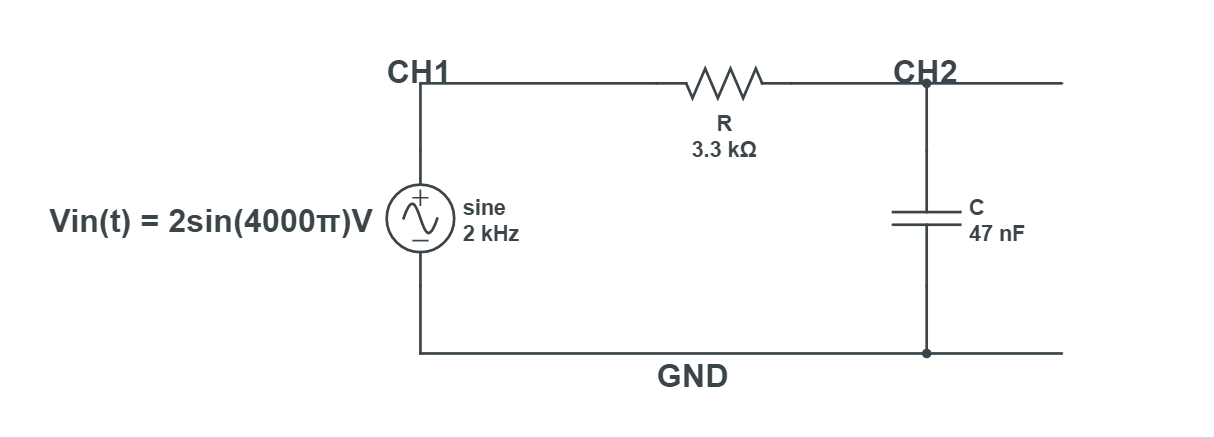
\includegraphics[width=1\textwidth]{6circuit.png}
\end{figure}

\subsubsection{a.}
In Figure 5, \( V_{in}\) (t) at Channel 1 ,\( V_0 \) (t) at Channel 2 is shown. The phase difference between the signals is measured as "65.\(\overline{45}\)  degrees" using the DSO cursors. The horizontal mode is set as the time for Figure 5.

\begin{figure}[H]
	\caption{\( V_{in}\) (t) at Channel 1 ,\( V_0 \) (t) at Channel 2  }
	\centering
	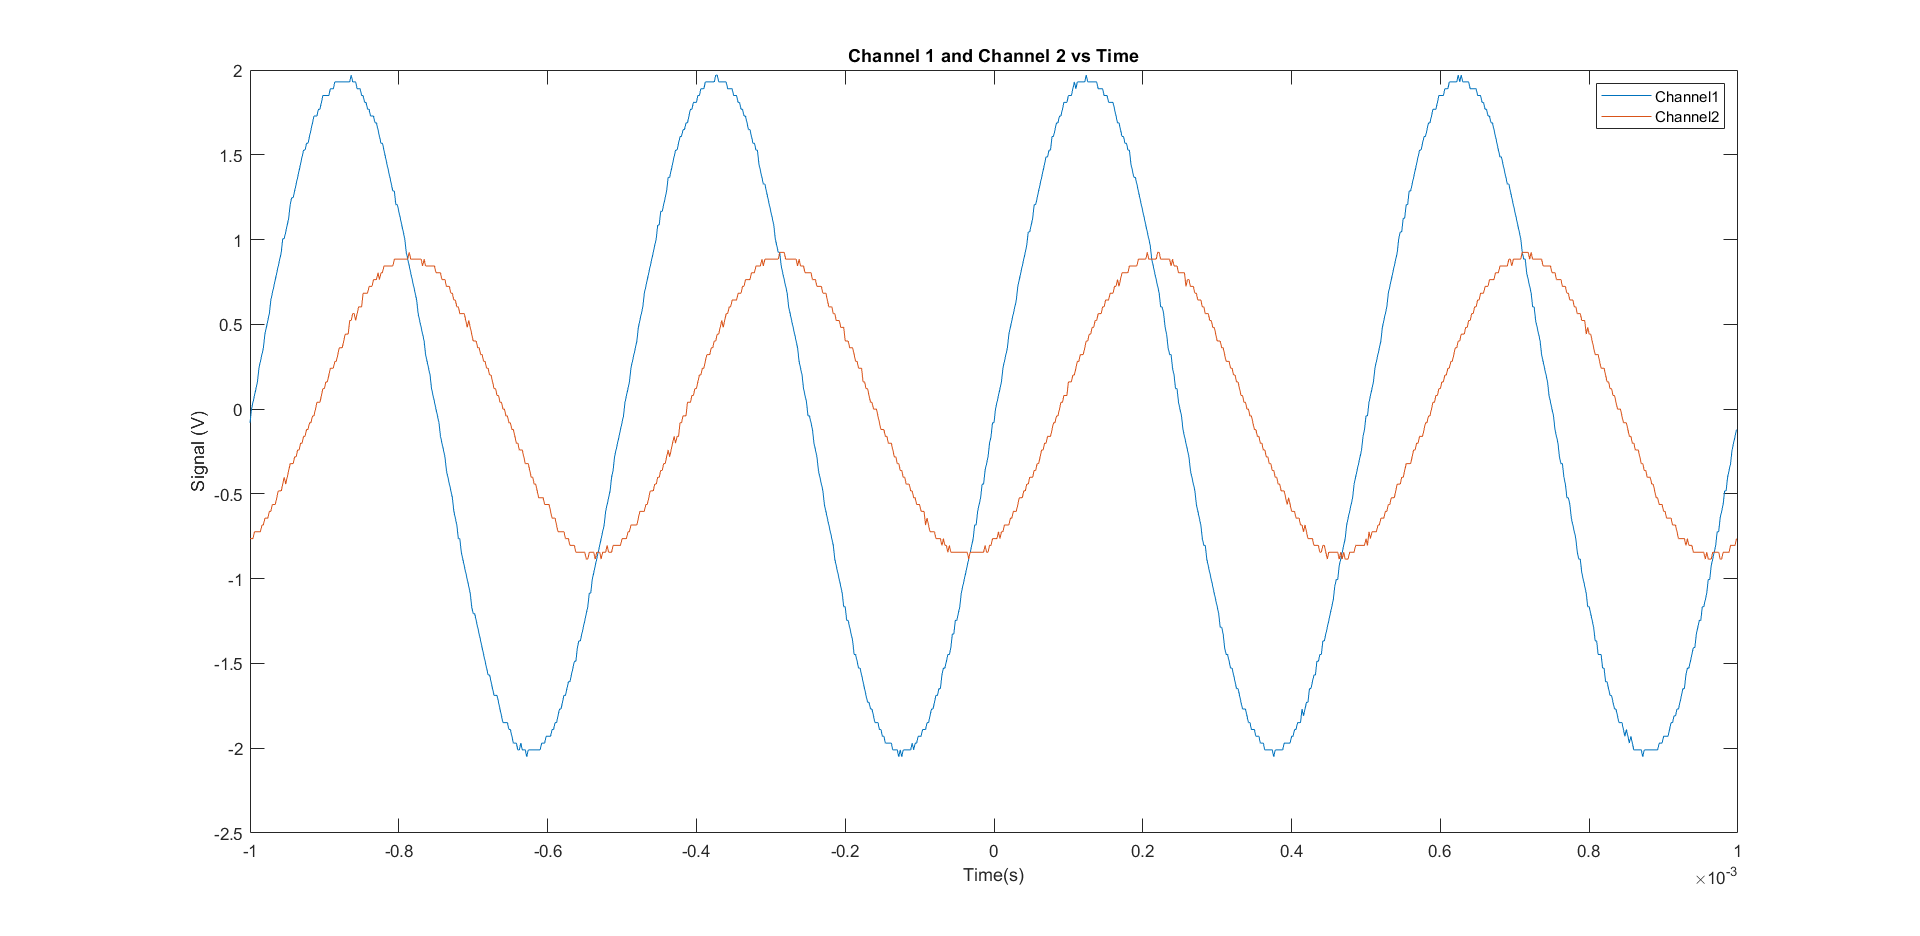
\includegraphics[width=1\textwidth]{6a.png}
\end{figure}

\subsubsection{b.}
In Figure 6, \( V_{in}\) at Channel 1 ,\( V_0 \) at Channel 2 is shown. The phase difference between the signals is measured as "63.78211805 degrees" using the DSO cursors Y1 and Y2. The difference between Y-axis interception points is denoted as A, and the difference between the boundary points is denoted as B. Then, using the \(arcsin({A}/{B})\) formula, the phase difference is determined. The XY mode is set as a time option for Figure 6.
\begin{figure}[H]
	\caption{\( V_{in}\) (t) at X axis \( V_0 \) (t) at Y axis  }
	\centering
	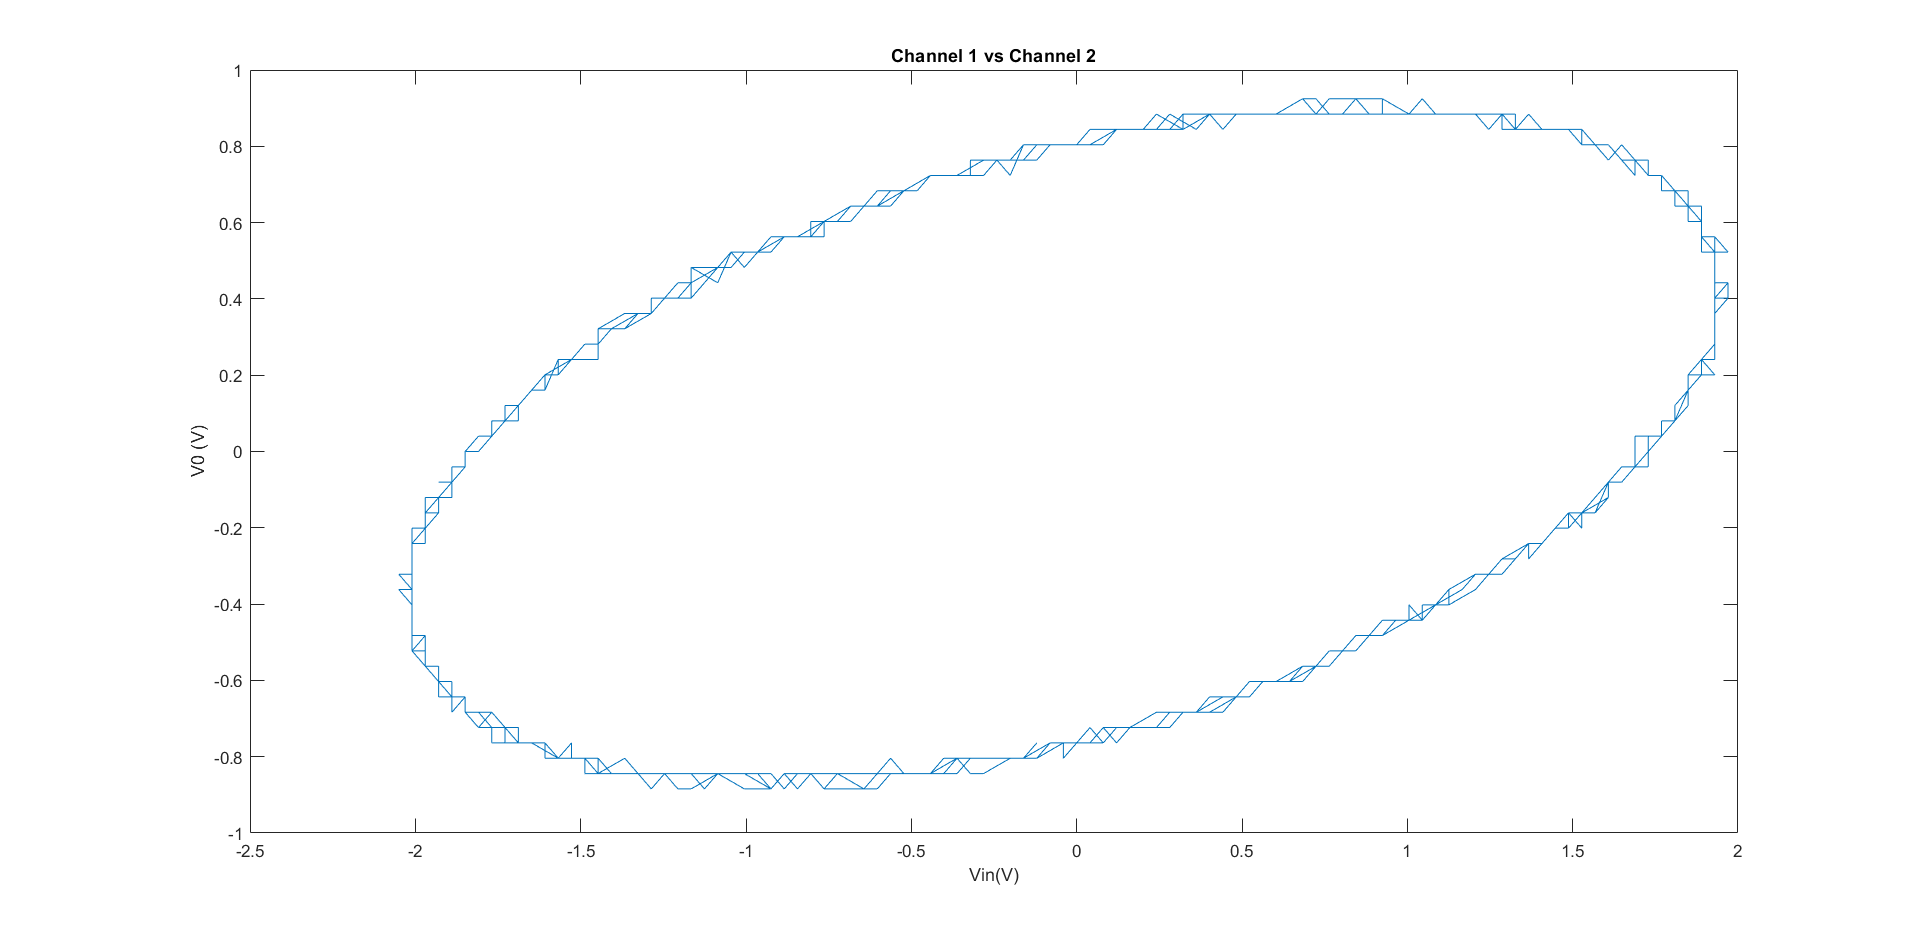
\includegraphics[width=1\textwidth]{6b.png}
\end{figure}

\subsection{Step 7}
The function waveform generator is adjusted 3 \(V_{pp}\) and frequency of 1.003 kHz. The "Channel 1" probes of the DSO are connected to the generators' output after making sure that the "Channel 2" is deactivated. Using the measurement tools on the oscilloscope, the properties of the autoscaled signal are measured. The  \(V_{pp}\) is displayed "3.06 Volts" . The period is displayed 998.8\( \mu \)s, and the frequency is 1.003 kHz.


\subsection{Step 8}
In this step, in addition to the setup at Step 7, the "Channel 2" probes are connected to the "Probe Comp" output and activated. Two waveforms were observed on the screen.
\subsubsection{a.}
Using the trigger and source buttons on the oscilloscope, "CH 1" is selected as the source. As a result, while the "Channel 1" signal is steady, the "Channel 2" signal becomes moving. 
\subsubsection{b.}
Using the trigger and source options on the oscilloscope, "CH 2" is selected as References. As a result, while the "Channel 2" signal is steady, the "Channel 1" signal becomes moving. 
\subsubsection{c.}
Small variations in the frequency of the output signal of the function generator are made. The signal slides are observed. To get two steady waveforms on the screen, the frequency is adjusted to "1.001,170 kHz". The reason why there are slides when we adjust the frequency higher or lower can be stated that the reference time frame of the sliding signal does not fit with the reference time frame of the trigger source signal.

\subsection{Step 9}
In this step the, circuit of Figure  7 is prototyped to the breadboard. The Channel 1 and Channel 2 probes are connected, as shown in the figure. After pressing the "Math" button, a third is observed in purple color. 
\begin{figure}[H]
	\caption{ The circuit diagram for Step 9  }
	\centering
	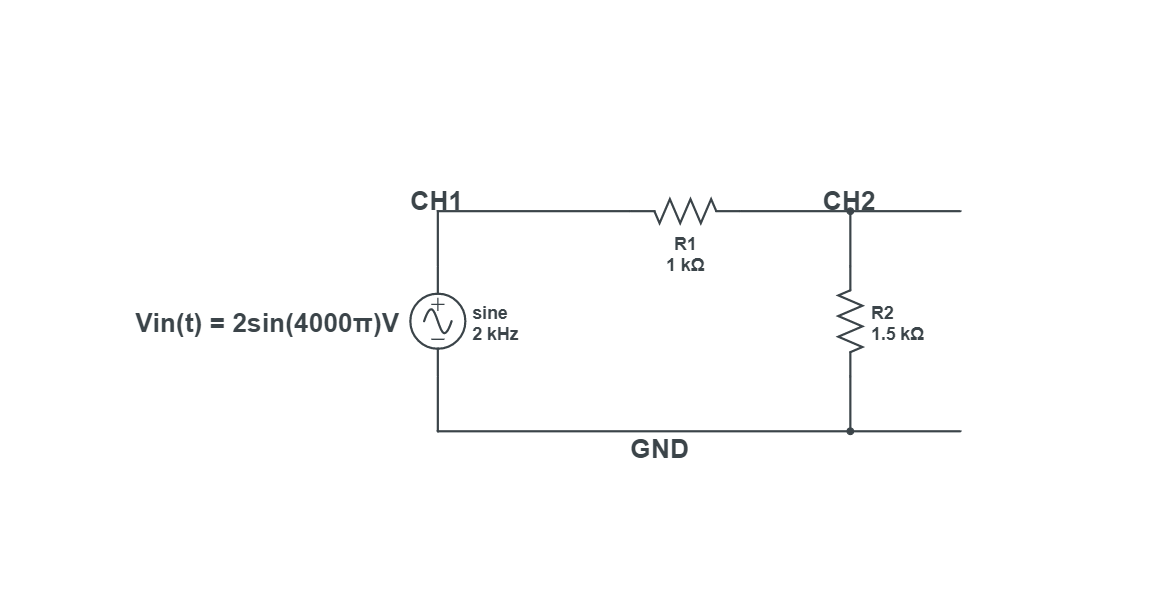
\includegraphics[width=1\textwidth]{9circuit.png}
\end{figure}

\subsubsection{a.}
Using the operator button, the "-" subtraction operation is selected. The subtraction of "Channel 2" from "Channel 1" is displayed on the oscilloscope screen as the third signal. 
\subsubsection{b.}
Using the operator button, the "+" addition operation is selected. The addition of "Channel 1" with "Channel 2" is displayed on the oscilloscope screen as the third signal. The data plot is given in Figure 8. It can be clearly seen that the amplitude of the resulting signal is the sum of the other two signals. 
\begin{figure}[H]
	\caption{ Channel Signals and Added Signal  }
	\centering
	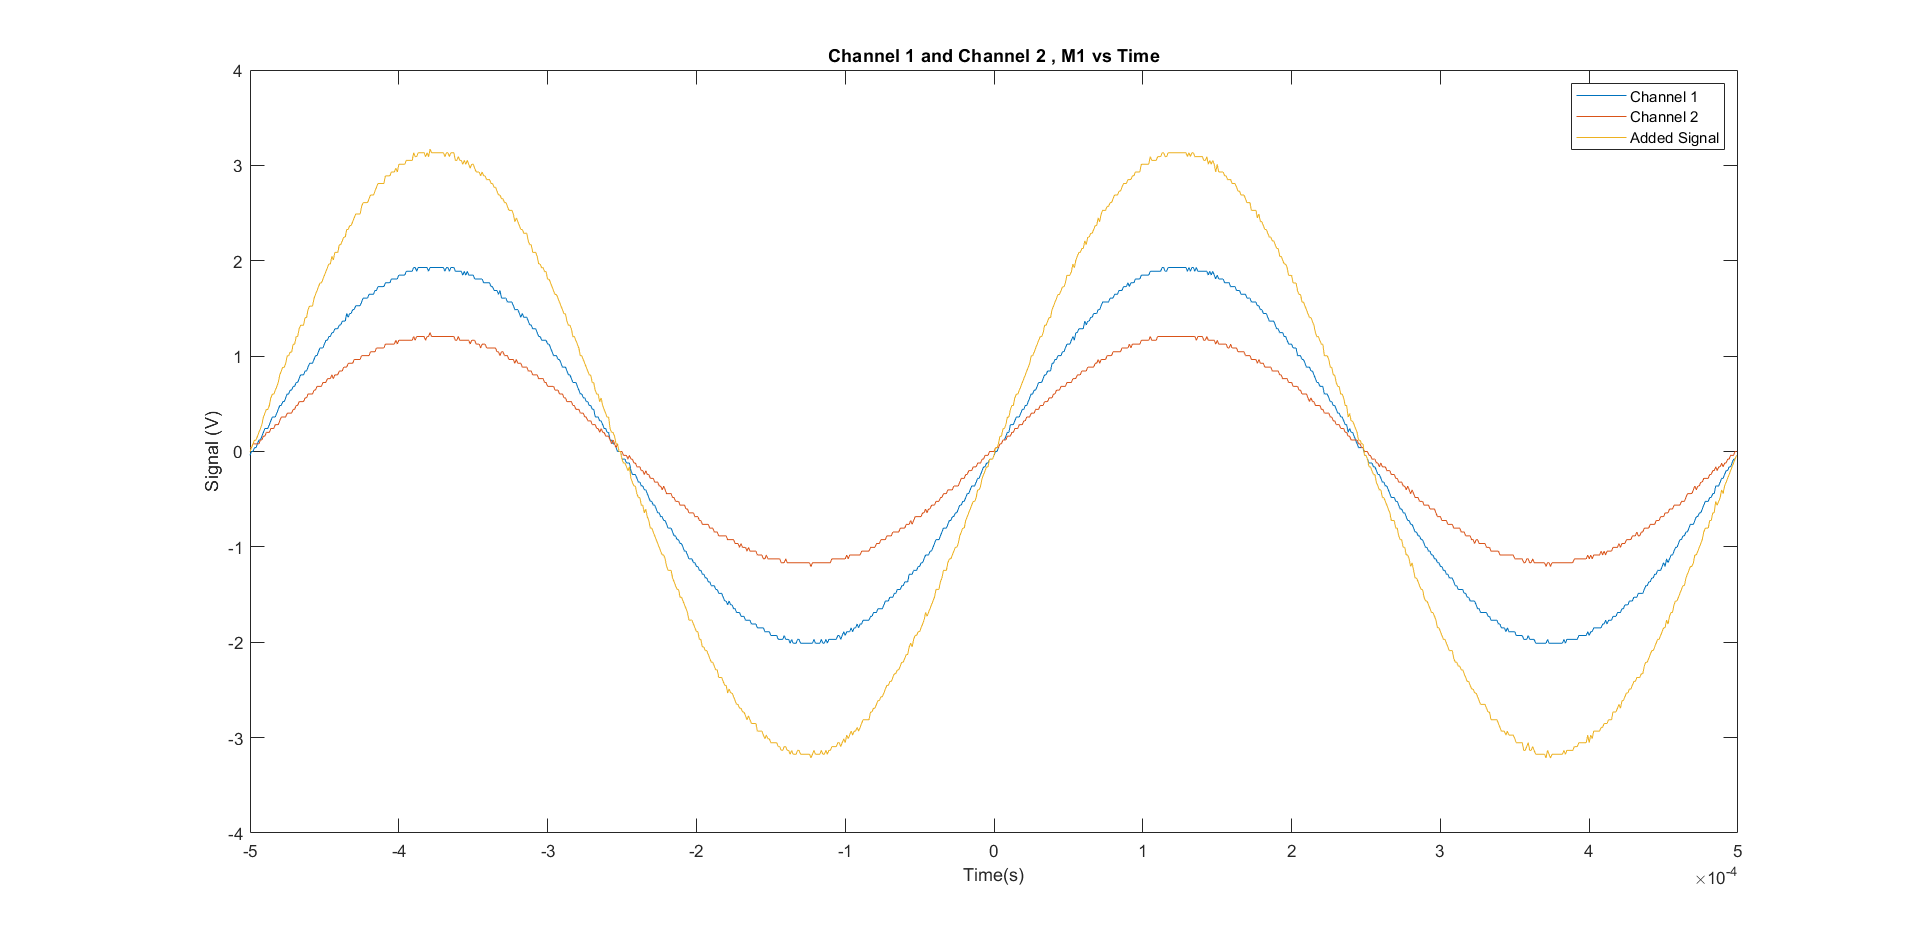
\includegraphics[width=1\textwidth]{9b.png}
\end{figure}


\section{Conclusion}
In conclusion, in experiment 2, "Signal Generators and Oscilloscopes," as students, we have learned how to use the signal generator and oscilloscopes instruments' behavior under nine steps. The scaling and movement properties of the oscilloscope channels are explored on a square waveform then the difference between "AC" and "DC" coupling methods are observed and explained. Also, inversion of the signal is observed then interpreted. The experiment repeated for the second channel, and the results are verified. Using cursor functions of the DSO, various measurements are made. The measurement features of the oscilloscope instrument are experienced. Different circuits are set and supplied by the signal generator, and the outputs are observed and plotted using DSO. The outputs of the function waveform generator and the prob comparison port of the oscilloscope are compared, and the trigger signal effect of the DSO is observed so that both signals are fit to the same time frame steady. Lastly, the mathematical operation ability is used to add and subtract the signals, then the results are observed.  In this experiment, as students, we have experimented with how to use signal generators and oscilloscopes.



\section*{Appendix I}
Total time spent on/during:
\begin{itemize}
	\item Pre-lab preparation: 1 hours (including the preliminary work and simulations) 
	\item Experimental work: 2 hours (hours spent in lab)
	\item Report writing: 8 hours 
\end{itemize}
%++++++++++++++++++++++++++++++++++++++++
% References section will be created automatically 
% with inclusion of "thebibliography" environment
% as it shown below. See text starting with line
% \begin{thebibliography}{99}
% Note: with this approach it is YOUR responsibility to put them in order
% of appearance.

%\begin{thebibliography}{99}

%https://tr.overleaf.com/latex/templates/sample-lab-report-for-u-of-r-phys-349/pgsyqngcyjxk

%\end{thebibliography}


\end{document}